\documentclass[12pt]{article} 

% \usepackage{ctex}
\usepackage{listings}
\usepackage{xcolor}
\usepackage{fontspec}
\usepackage{CJK}
\lstset{
    basicstyle          =   \sffamily,          % 基本代码风格
    keywordstyle        =   \bfseries,          % 关键字风格
    commentstyle        =   \rmfamily\itshape,  % 注释的风格,斜体
    stringstyle         =   \ttfamily,  % 字符串风格
    flexiblecolumns,                % 别问为什么,加上这个
    numbers             =   left,   % 行号的位置在左边
    showspaces          =   false,  % 是否显示空格,显示了有点乱,所以不现实了
    numberstyle         =   \ttfamily,    % 行号的样式,小五号,tt等宽字体
    showstringspaces    =   false,
    captionpos          =   t,      % 这段代码的名字所呈现的位置,t指的是top上面
    frame               =   lrtb,   % 显示边框
}

\lstdefinestyle{Python}{
    language        =   Python, % 语言选Python
    basicstyle      =   \ttfamily,
    numberstyle     =   \ttfamily,
    keywordstyle    =   \color{blue},
    keywordstyle    =   [2] \color{teal},
    stringstyle     =   \color{magenta},
    commentstyle    =   \color{red}\ttfamily,
    breaklines      =   true,   % 自动换行,建议不要写太长的行
    columns         =   fixed,  % 如果不加这一句,字间距就不固定,很丑,必须加
    basewidth       =   0.5em,
}
\bibliographystyle{plain}

\usepackage{graphicx}
\usepackage{subfigure}
\usepackage{float}
\usepackage{geometry}
\usepackage{enumerate}
\usepackage{indentfirst}
\setlength{\parindent}{2em}
\linespread{1.5}
\geometry{left=2.8cm,right=2.8cm,top=3cm,bottom=3cm}

\begin{document}

\title{Genetic Algorithm for Solving Traveling Salesman Problem}    
\author{Dongdong Geng-183139}
\maketitle
\abstract{
    The traveling salesman problem(TSP) is a combinatorial optimization problem with important practical significance. Genetic algorithm is one of the typical algorithms for solving traveling salesman problems. This paper first introduces the definition of traveling salesman problem and common algorithms, and elaborates the principle of genetic algorithm. In this paper, the reciprocal of the total length of the path is used as the fitness function to ensure that the understanding develops toward the optimization direction. Then select the sequential crossover operator to generate new individuals, which ensures the efficiency of the iteration. The mutation operator makes the algorithm simple and easy to use. Finally, two practical problems were solved when the number of cities was 10 and 20. Finally, the characteristics of the genetic algorithm are analyzed, and the direction of the improved algorithm is proposed.
}
%\section{Introduction}
%\section{Literature Review}
%\section{Problem Statement}
%\section{Mathematical Model}
%\section{Solution Algorithm}
%\section{Case Study}
%\section{Conclusion}

\section{Introduction}
% 遗传算法求解旅行商问题
The traveling salesman problem is a famous and classic problem in the study of optimal combination problems, and its research value is self-evident. There are practical applications for the traveling salesman problem, such as in traffic management planning. The main purpose of traffic management is to optimize the route of the vehicle in a complex geographic network structure to reduce transportation costs. Examples of application of the traveling salesman problem include: designing a safe, reasonable and efficient transportation network to reduce traffic congestion; how to plan better logistics routes, reduce the costs incurred by the operating industry, and reduce resource consumption.

Since the traveling salesman problem has such important practical significance, the algorithm for solving the traveling salesman problem will also develop. 
The earliest solution was linear programming, which later produced a variety of algorithms for solving traveling salesman problems. 
They can be roughly divided into precise algorithms, approximation algorithms, and intelligent algorithms. 
Precise algorithms: linear programming, dynamic programming, branch and bound; 
approximation algorithms include: interpolation, Clark \& Wright algorithm, spanning tree algorithm, nearest neighbor algorithm, probability algorithm, etc..
Many new intelligent algorithms have emerged in recent years. Such as simulated annealing, ant colony algorithm and genetic algorithm.

This article describes what a traveling salesman problem is, and then briefly describes some of the algorithms currently used to solve the traveling salesman problem. After that, it introduces in detail what is the genetic algorithm and the implementation process of the genetic algorithm. Then it describes how to use the genetic algorithm to solve the traveling salesman problem and actually applied it.
\section{Literature Review} 

% Since the traveling salesman problem has such important practical significance, the algorithm for solving the traveling salesman problem will also develop. 
% The earliest solution was linear programming, which later produced a variety of algorithms for solving traveling salesman problems. 
% They can be roughly divided into precise algorithms, approximation algorithms, and intelligent algorithms. 
% Precise algorithms: linear programming, dynamic programming, branch and bound; 
% approximation algorithms include: interpolation, Clark \& Wright algorithm, spanning tree algorithm, nearest neighbor algorithm, probability algorithm, etc..
% Many new intelligent algorithms have emerged in recent years. Such as simulated annealing, ant colony algorithm and genetic algorithm.
In the 1960s, Professor J.H. Holland of the University of Michigan began to recognize the similar relationship between biological genetic and natural evolution phenomena and artificial adaptive systems, and introduced biological genetic mechanisms into the research of artificial adaptive systems. In 1967, his student Bagley J.D. first proposed the term "genetic algorithm" and developed genetic operators such as replication, crossover, mutation, dominant, and inversion. In the 1970s, Professor Holland published the monograph "Adaptation in Nature and Artificial Systems", systematically expounded the basic theory and method of genetic algorithm, and proposed the basic theorem of genetic algorithm - the pattern theorem, which laid a theoretical foundation for the development of genetic algorithm. Based on the idea of ​​genetic algorithm, Dr. De. Jong of the United States conducted a large number of pure numerical function optimization calculation experiments on the computer and established the famous De.Jong five function test platform. In the 1980s, genetic algorithms began to be widely used in various fields. In 1980, Smith applied genetic algorithms to the field of machine learning; Bethke systematically studied the genetic algorithm of function optimization. In 1989, David Goldberg published "Genetic Algorithm in Search, Optimization and Machine Learning", which became the first monograph on genetic algorithms. In the 1990s, genetic algorithms entered a period of prosperity, and both theoretical research and applied research have become very hot topics. In particular, the application research of genetic algorithms is particularly active, and is widely used in the fields of combinatorial optimization, production scheduling, machine learning, image processing, artificial life, etc. Moreover, the ability to use genetic algorithms for optimization and rule learning is also significantly improved.

\section{Traveling Salesman Problem}
\subsection{Definition of Traveling Salesman Problem}
% 旅行商问题作为组合数学中一个古老的问题,虽然易于描述但目前为止尚未被彻底解决,
% 目前己将其归纳为所谓的NP完全问题类,其经典提法如下:
% 推销员要带一堆货物去己知的一些地方卖商品,从首发地出发后,需要将剩下
% 的各地都旅行一遍,然后回到首发地。问该推销员需要选择怎样的路线才能使得总线程最短(己知各城市间距离)。

% 假设城市数目n时,那么组合的路径数即为(n-1)!。
% 在城市的数目不多的情况下,要找到最佳路线显然并没有难度,
% 但当城市数目増大时,组合路线的数目将会呈现指数级数増长规律,这种程度将是无法计算的,也就是"组合爆炸问题"。
% 现在假定城市的数目为20个,因此组合路径数为(20-1)!,这个组合数目是相当大的,
% 即使利用计算机计算,以每秒检索1000万条线路的速度计算,也得耗费386年的时间。

% 基于改进的遗传算法求解TSP问题
Traveling salesman problem(TSP) is an ancient problem in combinatorial mathematics. 
Although it is easy to describe, it has not been completely solved so far. 
It has been summarized as the NP complete problem. 
The classic formulation is as follows: 
the salesman wants to bring a pile of goods. 
Some places that you know sell goods. 
After starting from the starting place, 
you need to travel the rest of the place and then return to the starting place. 
Ask the salesman what route to choose to make the total distances the shortest (distance between cities is known).

Assuming that the number of cities is $n$, then the number of combined paths is $(n-1)!$.
In the case of a small number of cities, 
it is obviously not difficult to find the best route.
However, when the number of cities is large, 
the number of combined routes will be exponentially long, 
which will be uncalculated,
which is called the combined explosion problem.
Now suppose that the number of cities is 20, so the number of combined paths is $(20-1)!$, 
the number of combinations is quite large.
Even with computer calculations, it takes 386 years to calculate the speed of retrieving 10 million lines per second.

% 旅行商问题的研究与应用
\subsection{Mathematical Description}
TSP is described in mathematical language as 
finding a path to travel and satisfies the following objective function:
\begin{equation}
    f(V)=\min \sum_{i=1}^{n-1} d\left(v_{i}, v_{i+1}\right)+d\left(v_{n}, v_{1}\right)
\end{equation}
Where $v_i$ is the city number $v_i\in N,1\leq v_i\leq n$, 
$d(v_i,v_j)$ represents the weight between the city $i$ and the city $j$ 
(may represent: distance, time and other expenses), 
if it is a symmetric TSP, then there is $d(v_i,v_j)=d(v_j,v_i)$.

Let $G=(V,E)$ be the weighted complete graph, $V\in N$ denote the vertex set, and $E$ denote the edge set.($d_{ij}>0,d_{ii}=0,i,j\in N$)

Suppose $x_{ij}$ is equal to 0 or 1.
\begin{equation}
x_{i j}=\left\{\begin{array}{l}{1, (i,j)\in L} \\ {0, (i,j)\notin L}\end{array}\right.
\end{equation}
$L$ is the solution sequence, then the mathematical model of TSP can be written as the following linear programming form:
\begin{equation}
    \min D(L)=\sum_{i \neq j} d_{i j} x_{i j}
\end{equation}
\begin{equation} 
    \sum_{i \in V, j \neq i} x_{i j}=1
\end{equation}
\begin{equation} 
    \sum_{j \in V, j \neq i} x_{i j}=1
\end{equation}
\begin{equation} 
    \sum_{i, j \in V} x_{i j}=|L| \quad L \subset E
\end{equation}

Where $|L|$ is the number of elements in the set L. 
Constraint (4) (5) constrains each vertex to have one and only traversal. 
Constraint (6) constrains Hamilton to do not have any sub-loops, 
and finds the one with the smallest weight among all Hamiltons that satisfy the condition.

\section{Genetic Algorithm}
\subsection{Genetic Algorithm Description}
% 遗传算法是一种随机的,以自然选择、基因遗传学原理为基础的并行搜索算法,
% 是一种不考虑初始信息的高效全局寻优算法,
% 该算法通过将问题的解集看成一个种群,利用选择操作、交叉操作、变异操作等,最后得到优良解。
% 具有全局寻优能力、较强的适应性、简单的计算过程、在非线性问题上有较强的鲁棒性、对问题没有特定限制、对搜索空间要求低、跟其他算法结合操作简单等特点,
% 在优化函数、处理图像、自动控制、经济预测和工程优化等方面有广泛的应用,在解决NP难题方面有广泛的应用。

% 基于旅行商问题的改进遗传算法研究
Genetic algorithm is a random parallel search algorithm based on natural selection and genetic genetics. 
It is an efficient global optimization algorithm that does not consider initial information. 
The algorithm considers the solution set as a population. 
Using a selection operation, a cross operation, a mutation operation, etc., 
an excellent solution is finally obtained.
It has global optimization ability, strong adaptability, simple calculation process, strong robustness on nonlinear problems, no specific restrictions on problems, low requirements on search space, simple operation combined with other algorithms, etc.. 
It has a wide range of applications in optimization functions, image processing, automatic control, economic forecasting and engineering optimization, and has a wide range of applications in solving NP-hard problems.

\subsection{Genetic Algorithm Steps}
%求解TSP的改进遗传算法 
Goldberg summarizes a unified and basic genetic algorithm and becomes the Basic Genetic Algorithms (SGA). 
SGA only uses three kinds of genetic operators: selection operator, crossover operator and mutation operator. 
The structure is simple and easy to understand. 
It is the dimension and foundation of other genetic algorithms.
The basic process of SGA is shown in Figure 1.

\begin{figure}[h]
    \centering
    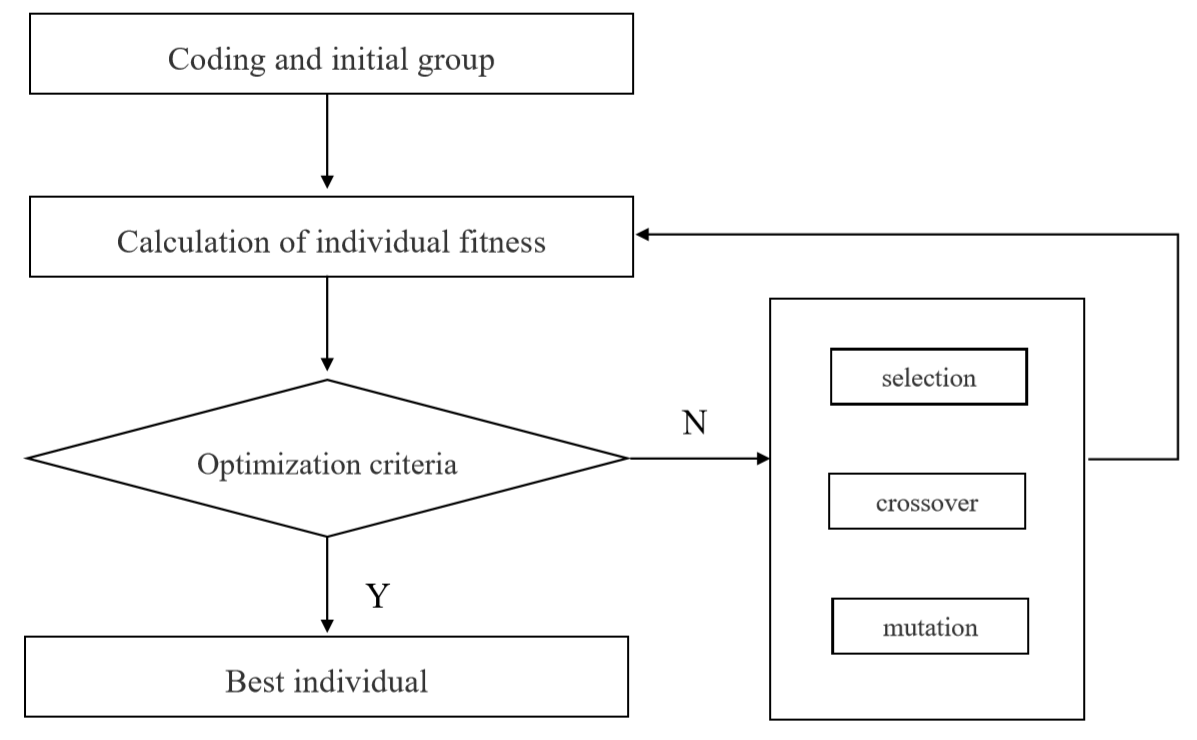
\includegraphics[width=0.8\textwidth]{process.png}
    \caption{Genetic algorithm}
\end{figure}

The specific algorithm steps are as follows:

Step1: Initialize to produce an initial population;

Step2: Individual evaluation, that is calculating the fitness of each individual in the population, and judging whether the optimization criteria are met.
If it is met, output the optimal solution or the satisfactory solution of the best individual and its representative, stop; otherwise, go to Step3;

Step3: Perform a selection operator according to the selection probability $p_s$, and select some individuals from the current population to enter the next generation population;

Step4: Perform a crossover operator according to the crossover probability $p_c$;

Step5: Perform a mutation operator according to the mutation probability $p_m$;

Step6: Generate a new generation of populations from crossovers and mutations, and turn to Step 2.

The optimization criteria of genetic algorithms generally have different determination methods depending on the problem. Generally, the following criteria can be used as the judgment conditions:
(1)Achieved a predetermined evolutionary algebra;
(2)The optimal individuals in the population have not improved after several consecutive generations;
(3)The optimal individual reaches a predetermined satisfactory solution.

\section{Genetic Algorithm for Solving TSP}
% 基于旅行商问题的改进遗传算法研究
\subsection{Coding}
Using natural number coding, each natural number represents a city. For example, an individual's chromosome can be represented by 1 2 3 4 5 6 7 , representing a route from city 1 through 2 3 4 5 6 7 and finally back to city 1.

In this paper, the optimization of the initial individual is based on the greedy algorithm, 
which uses its advantage of local optimization to generate new individuals. 
Select a city in a random way as the current city $C_0$, join the individual, search for the remaining cities, find the nearest city $C_1$ from the current city $C_0$, add $C_1$ to the individual and then use $C_1$ as the current city., 
repeated searches until all cities are added to the individual to form a complete route. Using this strategy to generate initial populations is also random, and it also improves the overall quality and speeds up the optimization.

\subsection{Fitness Function}
The individual's badness of the population is evaluated by fitness. The greater the fitness value, the better the individual. The fitness function is represented by the reciprocal of the total distance of the paths between cities in the traveling salesman problem.
The fitness function expression is as follows:
\begin{equation}
    f(x)=\frac{1}{\sum_{i=1}^{n-1} d\left(C_{i}, C_{i+1}\right)+d\left(C_{n}, C_{1}\right)}
\end{equation}

\subsection{Selection Operator}
The selection operation selects individuals from a determined probability in the original population to generate a new population. 
In order to preserve the excellent individuals in the group, this paper designs a new selection operator and adds the elite strategy.
when the selection of the generation of the population is generated, the proportional selection operator is used first
(The probability that each individual is selected is $P$. The upper generation $\alpha \times M$ individuals are selected.)
The parent populations are arranged in order of fitness size, and the $(1-\alpha)\times M$ individuals with better fitness are selected to insert the sub-populations, and finally $M$ individuals of the offspring are generated, wherein $\alpha$ is a selection factor.
The probability $P$ of an individual being selected is:
\begin{equation}
    P=\frac{f(x)}{\sum f(x)}
\end{equation}

\subsection{Crossover Operator}
This paper uses a sequential crossover operator, It first randomly selects two intersections in the parent, and then exchanges the intersections. The other positions are determined according to the relative order of the cities in the parent.
\[1\quad 2\quad |3\quad 4|\quad 5\quad 6 \quad \times \quad 1\quad 3\quad |5\quad 2|\quad 4\quad 6 \]
\[\downarrow \]
\[1\quad 5\quad |3\quad 4|\quad 2\quad 6\]

\subsection{Mutation Operator}
Although individual crossover increases population diversity, some good information may be lost, thus introducing a variation in fitness. The genetic position of the chromosome is changed correspondingly according to a certain probability. The mutation methods used in this paper include exchange mutation operators and in-position mutation operators. The specific operations are as follows:
\begin{enumerate}
    \item Exchange mutation operator. Two city numbers are randomly generated first, and the two city numbers are interchanged. If 3 and 5 are randomly generated from $[1, 6]$, determine the city number to be exchanged.
    \[1\quad 3\quad 6\quad 5\quad 4\quad 2 \longrightarrow 1\quad 5\quad 6\quad 3\quad 4\quad 2 \]
    \item In-position mutation operator. Randomly determine the two positions, and then reverse the order of the city numbers between the two positions. If positions 3 and 5 are generated from [1, 6].
    \[1\quad 3\quad 6\quad 5\quad 4\quad 2 \longrightarrow 1\quad 5\quad 4\quad 3\quad 6\quad 2\]
\end{enumerate}
\section{Case Study}
\subsection{Problem Statement}
In this paper, the genetic algorithm is used to solve the traveling salesman problem with the number of cities 10 and 20. The specific location of the city is shown in Figure 2.

\begin{figure}[h]
    \centering
    \subfigure[The number of cities is 10]{
    \begin{minipage}[b]{0.45\textwidth}
        \centering
        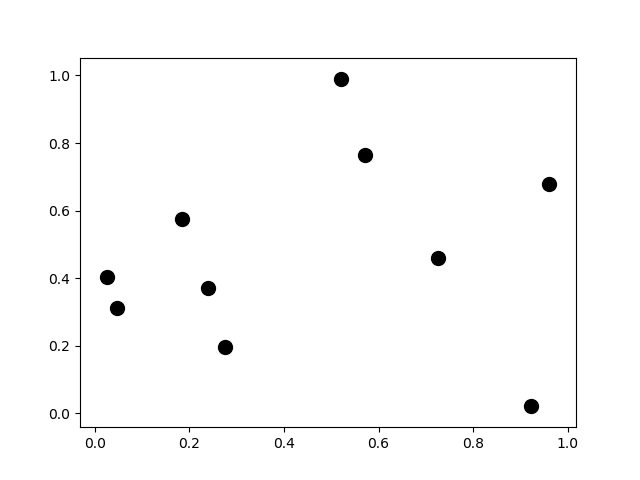
\includegraphics[width=0.8\textwidth]{10cities.png}
    \end{minipage}
    }
    \subfigure[The number of cities is 20]{
    \begin{minipage}[b]{0.45\textwidth}
        \centering
        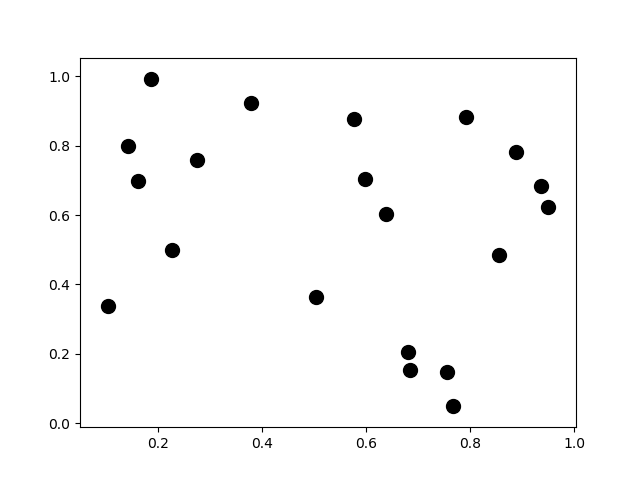
\includegraphics[width=0.8\textwidth]{20cities.png}
    \end{minipage}
    }
    \caption{Specific location of the city}
\end{figure}
\subsection{Result and Discussion}
Use genetic algorithm to find the path as shown in Figure 3.
The total distance of walking and the speed of iterative convergence of genetic algorithm are shown in Table 1.

\begin{figure}[h]
    \centering
    \subfigure[The number of cities is 10]{
    \begin{minipage}[b]{0.45\textwidth}
        \centering
        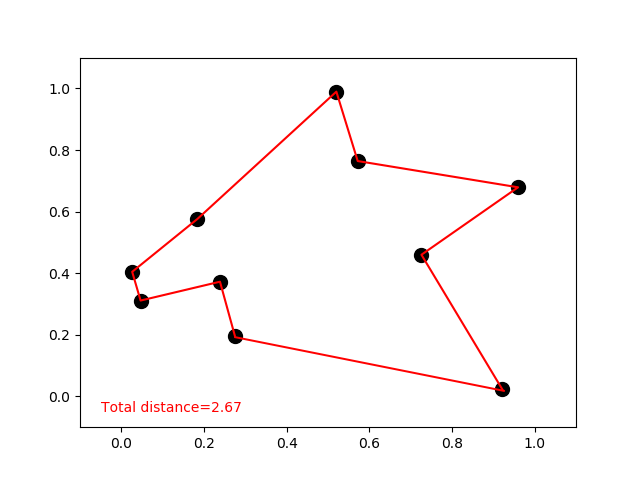
\includegraphics[width=0.8\textwidth]{10cities_path.png}
    \end{minipage}
    }
    \subfigure[The number of cities is 20]{
    \begin{minipage}[b]{0.45\textwidth}
        \centering
        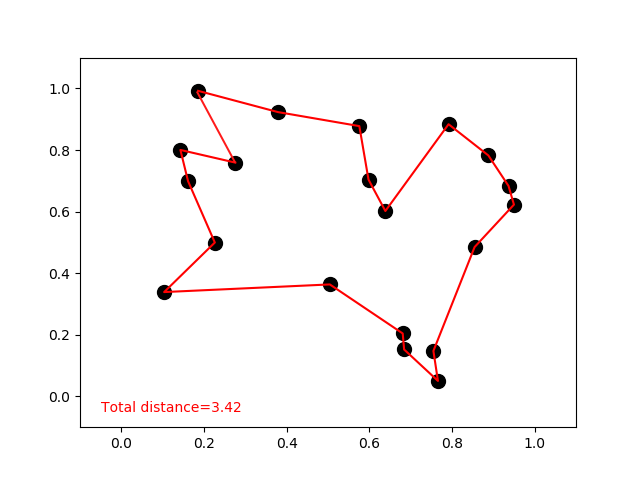
\includegraphics[width=0.8\textwidth]{20cities_path.png}
    \end{minipage}
    }
    \caption{Traveler walking path}
\end{figure}

\begin{table}[h]
    \centering
    \caption{Calculation results}
    \vspace{12pt}
    \begin{tabular}{lll}
    \hline
    Number of cities & Total distance & Number of iterations \\ \hline
    \hspace{2em}  10 &\hspace{2em}  2.67  & \hspace{3em}   11 \\
    \hspace{2em}   20 & \hspace{2em}   3.42  & \hspace{3em}   53 \\ \hline
    \end{tabular}
    \end{table}

It can be seen from the table that the genetic algorithm solves the traveling salesman problem quickly. When the number of cities is 10, 11 iterations can find the solution to the problem.
When the number of cities is 20, the number of iterations of the algorithm is 53. It is conceivable that when the number of cities increases, the number of times the algorithm needs to converge will increase sharply.

\section{Conclusion}
This paper briefly summarizes the methods to solve the traveling salesman problem and introduces the steps of the genetic algorithm. The coding, fitness function setting and various operator design when using the genetic algorithm to solve the traveling salesman problem are introduced in detail. Finally, the experiment shows that the genetic algorithm can solve the traveling salesman problem quickly. However, genetic algorithm tends to converge to local optimal solution, how to improve crossover operator, mutation operator and how to improve fitness function to improve genetic algorithm to make it iteratively to global optimal solution is the research direction of genetic algorithm to solve traveling salesman problem.
\newpage
\begin{thebibliography}{99}
    \bibitem{article1}Sun Hailei. \emph{An Improved Genetic Algorithm for TSP}[D]. Chongqing University. 2007
    \bibitem{article2}Wang Na. \emph{Improved Genetic Algorithem for TSP}[D]. Chongqing University. 2007
    \bibitem{article3}Zhang Zhanyun. \emph{Research on Improved Genetic Algorithm Based on Traveling Salesman Problem}[J]. 2017(07):19-21.
    \bibitem{article4}Yuan Hao. \emph{Research and application of traveling salesman problem}[D]. Nanjing University of Posts and Telecommunications. 2017.
    \bibitem{article5}Jiang Rong. \emph{Genetic Algorithm and its application in Travelling Salesman Problem}[D]. Hefei University of Technology. 2009.
    \bibitem{article6}Yu Fengrui. \emph{Improved Genetic Algorithm fer TSP}[D]. Inner Mongolia University Of Technology. 2016.
    \bibitem{article7}Cheng Rong. \emph{Genetic algorithm for traveling salesman problem}[J]. 2017(16):40-51.
    \bibitem{article8}Deng Lifang. \emph{Application Research of Genetic Algorithm for the Travelling Salesman Problem}[D]. Guangdong University of Technology. 2012.
    \bibitem{article9}Tan Jinhua. \emph{Eyolutionary Algorithms for Traveling Salesman Problems}[D]. Xidian University of Electronic Technology. 2008.
    \bibitem{article10}Wu Jun, Yan Lina. \emph{Solving TSP Problem Based on the Improved Genetic Algorithm}[J]. 2017(03):96-98.
\end{thebibliography}
\vspace{3.4cm}
Please excuse me!!\footnote{The reference format of the references is wrong because the use of \LaTeX is unskilled}
\newpage
\appendix
\section{Code}
\lstinputlisting[style=Python]{code.py}
\end{document}



